\documentclass[10pt,letterpaper,twocolumn]{article}
%\usepackage{setspace}
%\doublespacing
%\usepackage{iccv}
\usepackage{times}
\usepackage{epsfig}
\usepackage{graphicx}
\usepackage{setspace}
\usepackage{amsmath}
\usepackage{amssymb}
\usepackage{subfigure}
\usepackage{multirow}
\usepackage[linesnumbered,noend,ruled]{algorithm2e}
\usepackage{floatflt}
%\usepackage{floatrow}
%\floatsetup{footposition=caption}
%\newcommand{\subparagraph}{}

%\usepackage[small,compact]{titlesec}
%\usepackage[scriptsize,it]{caption}
%\DeclareCaptionFormat{myformat}{\hrulefill \newline #1#2#3}
%\captionsetup[figure]{format=myformat}

\newcommand{\mybeginlist}{\begin{list}{\labelitemi}{\setlength{\itemindent}{0.0in}}}
\newcommand{\mypar}[1]{\vspace{0.0in}\noindent{\bfseries#1}\hspace{0.5em}}
\newcommand{\myparnoskip}[1]{\noindent{\bfseries #1}\hspace{1em}}
\newcommand{\ie}{\emph{i.e.}, }
\newcommand{\eg}{\emph{e.g.}, }
\newcommand{\etc}{\emph{etc.}}
\newcommand{\etal}{, \emph{et al.}}

\newcommand{\squishlist}{
 \begin{list}{$\bullet$}
  { \setlength{\itemsep}{0pt}
     \setlength{\parsep}{1pt}
     \setlength{\topsep}{1pt}
     \setlength{\partopsep}{0pt}
     \setlength{\leftmargin}{1.0em}
     \setlength{\labelwidth}{1em}
     \setlength{\labelsep}{0.5em} } }

\newcommand{\squishlisttwo}{
 \begin{list}{$\bullet$}
  { \setlength{\itemsep}{0pt}
     \setlength{\parsep}{0pt}
    \setlength{\topsep}{0pt}
    \setlength{\partopsep}{0pt}
    \setlength{\leftmargin}{2em}
    \setlength{\labelwidth}{1.5em}
    \setlength{\labelsep}{0.5em} } }

%\titlespacing{\section}{0pt}{*0}{*0}
%\titlespacing{\subsection}{0pt}{*0}{*0}
%\titlespacing{\subsubsection}{0pt}{*0}{*0}

% vertical space reducers
\newcommand{\mysection}[1]{\vspace{-0.11in}\section{#1}\vspace{-0.09in}}
\newcommand{\mysectionstar}[1]{\vspace{-0.15in}\section*{#1}\vspace{-0.16in}}
\newcommand{\mysubsection}[1]{\vspace{-0.12in}\subsection{#1}\vspace{-0.11in}}
\newcommand{\mysubsectionstar}[1]{\vspace{-0.15in}\subsection*{#1}\vspace{-0.13in}}

\newcommand{\squishend}{
  \end{list}  }

% Include other packages here, before hyperref.

% If you comment hyperref and then uncomment it, you should delete
% egpaper.aux before re-running latex.  (Or just hit 'q' on the first latex
% run, let it finish, and you should be clear).
%\usepackage[pagebackref=true,breaklinks=true,letterpaper=true,colorlinks,bookmarks=false]{hyperref}
%\usepackage[pagebackref=true,breaklinks=true,colorlinks,bookmarks=false]{hyperref}
\usepackage[breaklinks=true,colorlinks,bookmarks=false]{hyperref}

\begin{document}

%\preprintfooter{}   % 'preprint' option specified.

\title{Affine Loop Optimization Using Modulo Unrolling in Chapel}
\author{Aroon Sharma}
%\subtitle{}
           
\maketitle

%\setcounter{page}{1}
%\vspace*{-9ex}
%\vspace*{-5ex}
\begin{abstract}

This paper presents component techniques essential for converting executables to a high-level intermediate representation (IR) of an existing compiler. The compiler IR is then employed for three distinct applications: binary rewriting using the compiler's binary back-end, vulnerability detection using source-level symbolic execution, and source-code recovery using the compiler's C backend. Our techniques enable complex high-level transformations not possible in existing binary systems, address a major challenge of input-derived memory addresses in symbolic execution and are the first to enable recovery of a fully functional source-code.
 %from an executable.
%First, the compiler's binary back-end is used to generate an output binary from the IR, yielding a binary rewriter. Second, a source-level symbolic execution tool is employed to detect vulnerabilities in the input executable. Third, the compiler's C backend is used to recover source-code for legacy binaries. This paper describes the first technique in literature to decompile an executable into an existing compiler's high-level intermediate representation
%

We present techniques to segment the flat address space in an executable containing undifferentiated blocks of memory. We demonstrate the inadequacy of existing variable identification methods for their promotion to symbols and present our methods for symbol promotion. We also present methods to convert the physically addressed stack in a binary (with a stack pointer) to an abstract stack (without a stack pointer). Our methods do not use symbolic, relocation, or debug information since these are usually absent in deployed binaries. 
%We show why the variable identification done by existing binary analysis tools is inadequate for their promotion to symbols in IR and present our methods for symbol promotion. We also show how to convert the physically addressed stack in a binary (with a stack pointer) to an abstract stack (without a stack pointer). Our methods do not use symbolic, relocation, or debug information since these are usually absent in deployed binaries. 
%Our methods are independent of the conventions of any particular compiler, OS, or language.
%We solve a  , a widely-used compiler infrastructure, , using variables instead
%Our techniques overcome challenges unique to executables: an explicitly addressed stack, the lack of function prototypes and the lack of symbols. 

We have integrated our techniques with a prototype x86 binary framework called SecondWrite that uses LLVM as IR. The robustness of the framework is demonstrated by handling binaries totaling more than a million lines of source-code, produced by two different compilers (gcc and Microsoft compiler), three languages (C, C++, and Fortran), two operating systems (Windows and Linux) and a real world program (Apache). 
%KLEE, a symbolic execution tool for detecting bugs in source code, is employed to symbolically execute the IR obtained from an input executable and achieves the same code coverage and detects same bugs as obtained through corresponding source-code. 
%The techniques presented in our paper greatly improve the readability and understandability of source-code recovered through our framework.
%SecondWrite accelerates un-optimized binaries by 45\% on average for our benchmarks, and further optimizes higly optimized binaries by 10\%, just by using standard optimizations present in LLVM.  
%We also present the impact of our techniques on automatic parallelization to exemplify the benefits and applications of a binary rewriter using a compiler IR.

\end{abstract}


\section{Introduction}\label{sec:intro} 

Message passing code generation is a difficult task for an optimizing compiler targeting a distributed memory architecture. These architectures are comprised of independent units of computation called locales, each with its own set of processors, memory, and address space. For programs executed on these architectures, data is distributed across various locales of the system, and the compiler needs to reason about locality in order to determine whether a data access is remote (requiring a message to another locale to request a data element) or local (requiring no message and accessing the data element on the locale's own memory). Each remote data memory access results in a message with some non-trivial run time overhead, which can drastically slow down a program's execution time. This overhead is caused by latency on the interconnection network and locality checks for each data element. Accessing multiple remote data elements individually results in this run time overhead being incurred multiple times, whereas if they are transferred in bulk the overhead is only incurred once. Therefore, aggregating messages improves performance of message passing codes. In order to transfer remote data elements in bulk, the compiler must be sure that all elements in question are remote before the message is sent. 

How a program's data is distributed and the program's data access patterns determine the degree of message aggregation that is possible. In this work, we consider three types of data distributions: Block, Cyclic, and Block Cyclic. In a Block distribution, elements of an array are mapped to locales evenly in a dense manner. In a Cyclic distribution, elements of an array are mapped in a round-robin manner across locales. In a Block Cyclic distribution, a blocksize parameter is specified and this number of elements is allocated to consecutive array indices in a round robin fashion. 

The vast majority of loops in scientific programs access data using affine array accesses. An affine array access is one that is a linear expression of the loop's index variables. Loops using affine array accesses are special because they exhibit regular access patterns within a data distribution. This information is used by the compiler to decide when message aggregation can take place. 

This paper presents a loop optimization for message passing code generation based on a technique called modulo unrolling. The optimization can be performed by a compiler to aggregate messages and reduce a program's execution time. Modulo unrolling in its original form, pioneered by \cite{barua1999maps}, was meant to target tiled architectures such as the MIT Raw machine, not distributed memory architecutres that use message passing. It has since been modified to apply to such machines in this work. Modulo unrolling used here works by unrolling an affine loop by a factor equal to the number of locales of the machine. If the arrays used in the loop are distributed cyclically, each array access is guaranteed reside on a single locale across all iterations of the loop. Using this information, the compiler can then aggregate remote array accesses into a single message before and after the loop. 

We demonstrate the modulo unrolling loop optimization in practice by implementing it in Chapel. Chapel is an explicitly parallel programming language developed by Cray Inc. that falls under the Partitioned Global Address Space (PGAS) memory model. Here, a system's memory is abstracted to a single global address space regardless of the hardware implementation and is then logically divided per locale and thread of execution. By doing so, locality of reference can easily be exploited no matter how the system architecture is organized. The Chapel compiler is an open source project used by many in industry and academic settings. The language contains many high level features such as zippered iteration that greatly simplify the implementation of modulo unrolling into the language. 
\section{Intuition Behind Message Aggregation With An Example}\label{sec:motivation_for_aggregation} 

In Chapel, a program's data access patterns and the programmer's choice of data distribution greatly influence the program's runtime and communication behavior. This section presents an example of a Chapel program with affine array accesses that can benefit from message aggregation. It also serves to present the intuition behind how modulo unrolling WU will be used in message aggregation. 

The intuition behind why modulo unrolling is helpful for message aggregation in message passing machines is as follows. Message aggregation requires knowledge of precisely which elements must be communicated between locales. Doing so requires a statically disambiguated known locale for every array access, even when that array access refers to a varying address. For example, in a loop $A[i]$ refers to different memory addresses during each loop iteration. Modulo unrolling ensures such a known, predictable locale number for each varying array access. This enables such varying accesses to be aggregated and sent in a single message. We explain our method of doing so in Sections \ref{sec:transformation} and \ref{sec:adaptation_in_chapel}.

\begin{figure}
\begin{center}
\includegraphics[width=\linewidth]{./Figures/jacobi}
\caption{Chapel code for the Jacobi-2D computation over an 8 x 8 two dimensional array. Arrays $A$ and $A_{new}$ are distributed with a Cyclic distribution and their declarations are not shown. During each iteration of the loop, the current array element $A_{new}[i, j]$ gets the average of the four adjacent array elements of $A[i, j]$.}
\label{jacobi_code}
\end{center}
\end{figure}

\begin{figure}
\begin{center}
\includegraphics[width=\linewidth]{./Figures/aggregation}
\caption{Illustration of message aggregation for the $A[i, j-1]$ affine array access of the Jacobi-2D relaxation computation with respect to locale 3. The region \textit{LoopSpace} follows from Figure \ref{jacobi_code}. The striped squares are the elements of $A$ that have been aggregated. This same procedure occurs on each locale for each affine array access that is deemed to be remote for all iterations of the loop. For the whole 8 x 8 Jacobi-2D calculation, 144 remote gets containing one element each are necessary without aggregation, but only 16 remote gets containing nine elements each are necessary with aggregation.}
\label{aggregation}
\end{center}
\end{figure}

Consider the Chapel code for the Jacobi-2D computation shown in Figure \ref{jacobi_code}, a common stencil operation that computes elements of a two-dimensional array as an average of that element's four adjacent neighbors. We assume that arrays $A$ and $A_{new}$ have already been distributed using a Cyclic distribution over four locales. On each iteration of the loop, five array elements are accessed in an affine manner: the current array element $A_{new}[i, j]$ and its four adjacent neighbors $A[i+1, j]$, $A[i-1, j]$, $A[i, j+1]$, and $A[i, j-1]$. The computation will take place on the locale of $A_{new}[i, j]$, the element being written to. If arrays $A$ and $A_{new}$ are distributed with a Cyclic distribution as shown in Figure \ref{cyc_dist}, then it is guaranteed that $A[i+1, j]$, $A[i-1, j]$, $A[i, j+1]$, and $A[i, j-1]$ will not reside on the same locale as $A_{new}[i, j]$ \textbf{for all iterations of the loop}. Therefore, these remote elements need to be transferred over to $A_{new}[i, j]$'s locale in four separate messages during every loop iteration. For large data sets, transferring four elements individually per loop iteration drastically slows down the program because the message overhead is incurred many times. 

We observe that message aggregation of remote data elements is possible over the entire loop for the Jacobi-2D example. Aggregation will reduce the number of times the message overhead is incurred during the loop. When the data is distributed using a Cyclic distribution, all array accesses (including remote accesses) exhibit a predictable pattern of locality. 

Figure \ref{aggregation} illustrates this pattern in detail for loop iterations that write to locale 3. During these iterations ($(i, j) = (2, 2), (i, j) = (4, 2)$, etc.), there are two remote accesses from locale 1 and two remote accesses from locale 2. The remote accesses from locale 1 correspond to the $A[i, j+1]$, and $A[i, j-1]$ affine array accesses in Figure \ref{jacobi_code}. If we highlight all the remote data elements corresponding to the $A[i, j-1]$ access that occur for loop iterations that write to locale 3, we end up with the array slice $A[2..7$ $by$ $2, 1..6$ $by$ $2]$, which contains the striped elements in Figure \ref{aggregation}. This array slice can be communicated from locale 1 to a buffer on locale 3 before the loop executes in a single message. Then, during the loop, all $A[i, j-1]$ accesses can be replaced with accesses to the local buffer on locale 3. 

The previous paragraph showed how aggregation occurs for the $A[i, j-1]$ affine array access on loop iterations that write to locale 3. This same procedure applies to the other three remote accesses for locale 3. In addition, this same procedure applies to loop iterations that write to the remaining locales. Finally, we claim that this optimization can also be applied to the Block Cyclic distribution, as the data access pattern is the same for elements in the same position within a block. 

In this example, we chose to perform message aggregation with respect to the element that is written to during the loop. However, this is not always the best choice for all programs. To get better communication performance, we would like to assign loop iterations to locales with the most affine array accesses that are local. The result of this scheme is that elements that are written to during the loop may be the ones that are aggregated before the loop. If so, it is necessary to write these elements from the local buffers back to their remote locales. This is done in a single aggregate message after the loop body has finished.\footnote{In Chapel, the programmer has some control over assigning loop iterations to locales. Therefore, our optimizations uses the programmer's assignment of loop iterations to locales when performing message aggregation.} 

If arrays $A$ and $A_{new}$ are instead distributed using Chapel's Block or Block Cyclic distributions as shown in Figure \ref{block_dist} and Figure \ref{block_cyc_dist} respectively, the program will only perform remote data accesses on iterations of the loop where element $A_{new}[i, j]$ is on the boundary of a block. As the block size increases, the number of remote data accesses for the Jacobi-2D computation decreases. For the Jacobi-2D computation, it is clear that distributing the data using Chapel's Block distribution is the best choice in terms of communication. Executing the program using a Block distribution will result in fewer remote data accesses than when using a Block Cyclic distribution. Similarly, executing the program using a Block Cyclic distribution will result in fewer remote data accesses than when using a Cyclic distribution. 

It is important to note that the Block distribution is not the best choice for all programs using affine array accesses. Programs with strided access patterns that use a Block distribution will have poor communication performance because accessed array elements are more likely to reside outside of a block boundary. For these types of programs, a Cyclic or Block Cyclic distribution will perform better. Section \ref{sec:data_distributions} explained several reasons why the programmer may have chosen a Cyclic or Block Cyclic distribution.

\begin{comment}
When $(i, j) = (2, 2)$, $A_{new}[2, 2]$ resides on locale 3. $A[2, 1]$ corresponds to the $A[i, j-1]$ access during this iteration, and it resides remotely on locale 1. If we now look at the next iteration where $A_{new}[i, j]$ resides on locale 3 (the next cycle, which is $(i, j) = (4, 2)$), we see that $A[4, 1]$ also resides on locale 1. We notice a pattern that all remote data accesses with respect to locale 3 corresponding to the $A[i, j-1]$ access in the loop \textbf{form an array slice $A[2..7$ $by$ $2, 1..6$ $by$ $2]$}, which we can aggregate with a single GET call and bring into $buf$\_$north$ on locale 3 before the loop begins. The array slice contains strided accesses of 2 in both the $i$ and $j$ dimensions, denoted using the Chapel keyword \textit{by} within the array slice. 
\end{comment}





\section{Modulo Unrolling}\label{sec:modulo_unrolling}

This section describes modulo unrolling. 
\section{Chapel Zippered Iteration}\label{sec:zippered_iteration}

Iteration is a widely used language feature in the Chapel programming language. Chapel iterators are blocks of code that are similar to functions and methods except that iterators can return multiple values back to the call site with the use of the \textit{yield} keyword instead of \textit{return}. Iterators are commonly used in loops to traverse data structures in a particular fashion. For example, an iterator $fibonacci(n: int)$ might be responsible for yielding the first $n$ Fibonacci numbers. This iterator could then be called in a loop's header to execute iterations 0, 1, 1, 2, 3, and so on.  Arrays themselves are iterable in Chapel by default. 

Chapel allows multiple iterators of the same size and shape to be iterated through simultaneously. This is known as \textit{zippered iteration} \cite{chamberlain2011user}. When zippered iteration is used, correpsonding iterations are processed together. On each loop iteration, an $n$-tuple is generated, where $n$ is the number of items in the zippering. The $d^{th}$ component of the tuple generated on loop iteration $j$ is the $j^{th}$ item that would be yielded by iterator $d$ in the zippering. Figure~\ref{zippered_iteration} shows an example of zippered iteration used in a Chapel \textbf{for} loop. 

Zippered iteration can be used with either sequential \textbf{for} loops or parallel \textbf{forall} loops in Chapel. Parallel zippered iteration is implemented in Chapel using leader-follower semantics. That is, a leader iterator is responsible for creating tasks and dividing up the work to carry out the parallelism. A follower iterator performs the work specified by the leader iterator for each task and generally resembles a  serial iterator. 

\subsection{Chapel Array Slicing}\label{sec:array_slicing}

Chapel supports another useful language feature known as \textit{array slicing}. This feature allows portions of an array to be accessed and modified in a succicnt fashion. For example, consider two arrays $A$ and $B$ containing indices from $1..10$. Suppose we wanted to assign elements $A[6]$, $A[7]$, and $A[8]$ to elements $B[1]$, $B[2]$, and $B[3]$ respectively. We could achieve this in one statement by writing $B[1..3] = A[6..8]$. Here, $A[6..8]$ is a slice of the original array $A$, and $B[1..3]$ is a slice of the original array $B$. An array slice can support a range of elements with a stride in some cases. For example, in the previous example, we could have made the assignment $B[1..3] = A[1..6$  $by$  $2]$. This would have assigned elements $A[1]$, $A[3]$, and $A[5]$ to elements $B[1]$, $B[2]$, and $B[3]$ respectively. Since all array slices in Chapel are arrays themselves, array slices are also iterable. 

Together, array slicing and parallel zippered iteration can express any parallel affine loop in Chapel that uses affine array accesses. Each affine array access is replaced with a correpsonding array slice which produces the same elements as the orignal loop. Consider the code fragment in Figure \ref{affine_loop}a. There are two affine array accesses $A[i]$ and $B[i+2]$ in Figure \ref{affine_loop}a. The loop is written in a standard way where the loop induction variable $i$ takes on values from 1 to 10. Because the loop is a \textbf{forall} loop, loop iterations are not guaranteed to complete in a specific order. This loop assigns elements of array $B$ to $A$ such that the $i^{th}$ element of $A$ is equal to the $(i+2)^{th}$ element of $B$ after the loop finishes. In Figure \ref{affine_loop}b, the same loop is written using zippered iteration. The loop induction variable $i$ no longer needs to be specifed, and each affine array access has been replaced with an array slice in the zippering of the loop header. It is possible to transform an affine loop in this fashion even when an affine array access has a constant factor multiplied by the loop induction variable. The resulting array slice will contain a stride equal to the constant factor.\footnote{Question by Aroon: Is it true to say that any affine array access can be transformed using the way described here? What if the access was something like $A[2i+3j]$?}

Because any parallel affine loop can be transformed to an equivalent parallel loop that uses zippered iteration, we observe a natural place in the Chapel programming language in which to implement modulo unrolling: the leader and follower iterators of the Cyclic and Block Cyclic distribution. 

\begin{figure}
	\begin{center}
	\includegraphics[scale=0.65]{./Figures/zippered_iteration}
	\caption{(a) Chapel code fragment showing a loop using zippered iteration. A tuple of loop index variables equal to the number of items in the zippering is declared in the loop header. If the variable $j$ corresponds to the current loop iteration, $i$ corresponds to the $j^{th}$ element in the range $1..5$, and $f$ corresponds to the $j^{th}$ element in the iterator $fibonacci(5)$. The \textit{zip} keyword tells the loop header which items to iterate over using zippered iteration. (b) Program output of the code fragment in Figure~\ref{zippered_iteration}a.}
	\label{zippered_iteration}
	\end{center}
\end{figure}

\begin{figure}
	\begin{center}
	\includegraphics[scale=0.60]{./Figures/affine_loop}
	\caption{(a) Original loop written using a single loop induction variable $i$ ranging from 1 to 10. (b) The same loop written using zippered iteration. Instead of a loop induction variable and a range of values to denote the loop bounds, two array slices containing 10 elements each are specified.}
	\label{affine_loop}
	\end{center}
\end{figure}
\section{Cyclic Distribution with Modulo Unrolling}\label{sec:cyclic_modulo}

For the Cyclic distribution, only the follower iterator needs to be modified.\footnote{Aroon's comment: I am still working on a clear way to explain how modulo unrolling is implemented in both distributions without going into too much detail. Any suggestions on how I should do this?}
\section{Block Cyclic Distribution with Modulo Unrolling}\label{sec:block_cyclic_modulo}

For the Chapel Block Cyclic implementation, both the leader and follower iterators have been modified to support the modulo unrolling optimization. Modulo unrolling, unaltered, is not compatible with the Block Cyclic distribution because consecutive array elements can reside on the same locale, which destroys the static locality information that we were able to use in the Cyclic distribution. The Block Cyclic leader iterator is now modified to choose slices of work such that the new "stride" is equal to the product of the block size and the cycle size. This way, when the work is passed to the follower iterator, elements that are in the same position within each block are guaranteed to be on the same locale. The follower iterator of the Block Cyclic distribution can now perform modulo unrolling in the same way as the Cyclic distribution. 


\section{Results} 
\label{sec:results}
%\vspace{-2ex}
Fig~\ref{fig:appTable} lists all the benchmarks which have been successfully evaluated with SecondWrite prototype. It includes the complete SPEC2006 benchmark suite, benchmarks from other suite and a real world program, Apache server. As evident from Fig~\ref{fig:appTable}, SecondWrite is able to correctly handle binaries from three different programming languages (C, C++, Fortran), two different compilers (gcc and Visual studio) and two different OS (Linux and Windows), demonstrating the robustness of our techniques. Benchmarks on Linux are compiled with gcc v4.4.1 (O0 (No optimization) and O3 (Full optimization) flags) without any symbolic or debug information. Results are obtained for \emph{ref} datasets
on a 2.4GHz 8-core Intel Nehalem machine running Ubuntu. Windows benchmarks are compiled with Microsoft Visual Studio compiler (O0 (No optimization) and O2 (Maximum optimization) flags). \emph{Only the C and C++ programs are included for Windows since VisualStudio does not compile Fortran}. In the case of Apache server, we tested a \emph{http} server with the rewritten binary. Apache server, being an interactive program, is not amenable to performance analysis like other benchmarks; hence we only provide its static results.
%It is a diverse set of programs totalling more than 400K lines of code. 
%We were also able to correctly apply the standard suite of LLVM transformation passes without any changes.  
%A subset of \emph{SPEC} benchmarks, \emph{OpenMP} benchmarks and a few real world programs are evaluated to substantiate the performance of our rewriter. 
\begin{figure}[t]
{
%\vspace{-0.2in}
\centering
%\psfig{figure=figures/plots/runtimeFinal.eps,width=5.5in} }
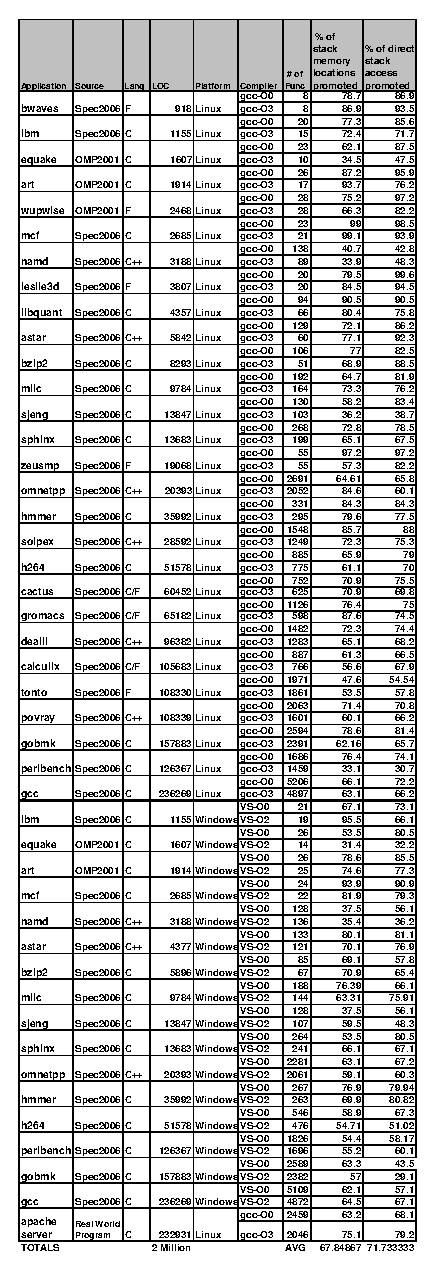
\includegraphics [width=0.7\linewidth] {figures/EPS/appTablenew2.eps} 
%\vspace{-3ex}
\caption { \textit{Benchmarks Table}}
\label{fig:appTable}
}
\vspace{-2ex}
\end{figure}
 

%%\begin{figure}[t]
%\vspace{-0.5in}
%\centering
%\psfig{figure=figures/plots/runtimeFinal.eps,width=5.5in} }
%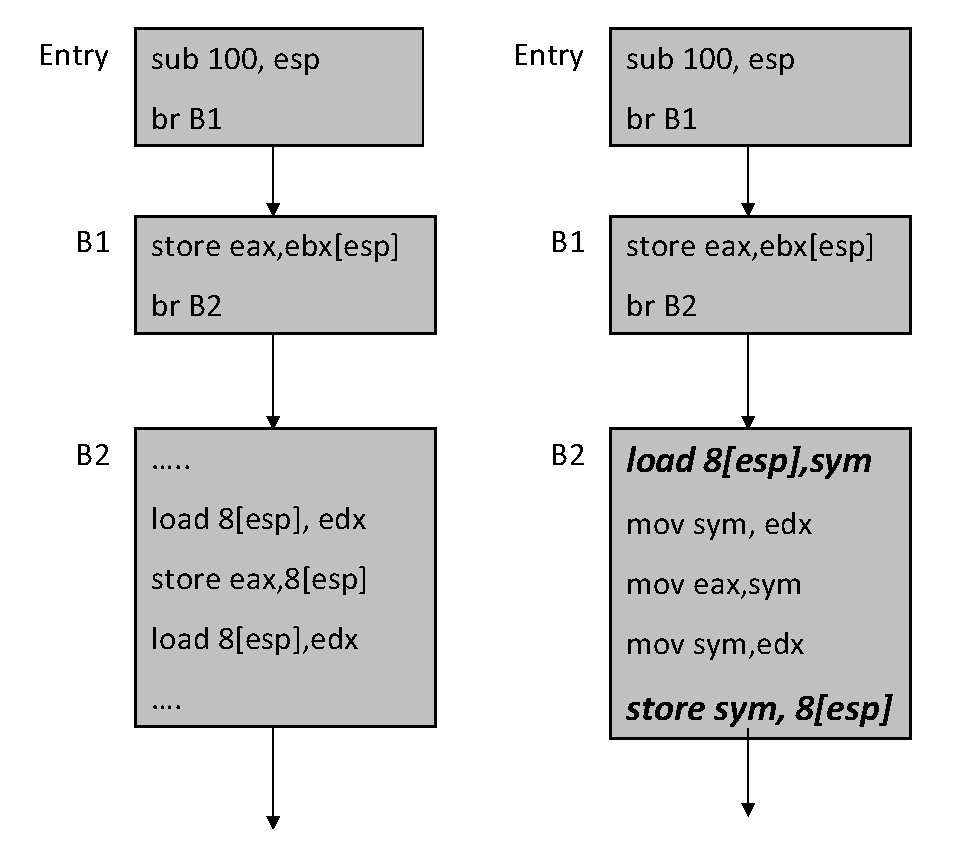
\includegraphics [width=0.5\linewidth] {figures/EPS/cfgex.eps} 
%\tiny{
%\caption { \textit{Stack layout in a binary}}
%}
%\label{fig:stack-layout}
%\end{figure}

\begin{figure}[b]
{
\vspace{-2ex}
\centering
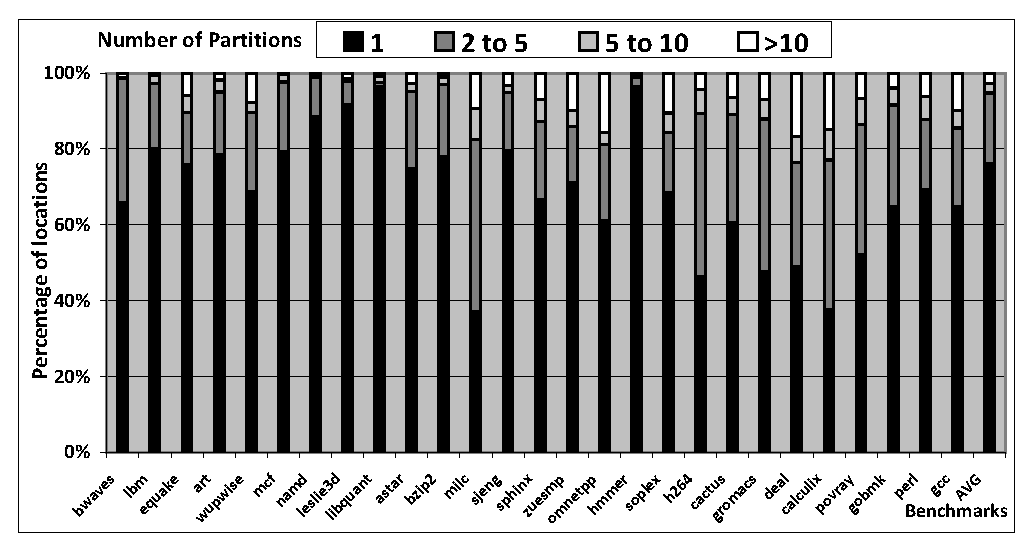
\includegraphics[width=0.8\linewidth]{figures/EPS/partition-visualization-2.eps}
%\vspace{-3ex}
\caption{\textit{Partition algorithm visualization }}
\label{fig:PartResult}
}
%\hfill
\vspace{-3ex}
\end{figure}




%\begin{figure}[t]
%{
%\centering
%\begin{minipage}{.6\linewidth}
%{
%\centering
%\includegraphics[width=0.5\linewidth]{figures/EPS/pathcfg.eps}
%\caption{\textit{Path dependent promotion. Second operand in the instruction is the destination of the instruction. }}
%\label{fig:PromExample}
%}
%\vspace{-0.1in}
%\end{minipage}
%%\hfill
%\begin{minipage}{0.3\linewidth}
%{
%\centering
%\includegraphics[width=0.3\linewidth]{figures/EPS/partitioncfg.eps} 
%\caption{\textit{Motivation for partition}}
%\label{fig:PartExample}
%}
%\vspace{-0.1in}
%\end{minipage}
%}
%\vspace{-0.2in}
%\end{figure}

\subsection{Static characteristics}
Fig~\ref{fig:appTable} displays the static characteristics of symbol promotion techniques - the percentage of stack memory locations promoted to symbols and the percentage of direct stack memory accesses promoted to symbol accesses in the IR and in the recovered source-code. The results depict that on average, 67\% of stack locations are promoted to symbols resulting in promotion of 72\% of direct stack accesses. For the remaining memory operations, the net benefit for promotion didn't meet the corresponding threshold. Theoretically, our framework can achieve \emph{100\% symbol promotion} if the promotion threshold is ignored, but this leads to high overhead in the rewritten binaries due to \emph{Promoting Loads} and \emph{Promoting Stores}. The development of more advanced alias analysis would improve results of our symbol promotion without adversely affecting the performance.

\begin{figure*}[t]
{
\vspace{-0.3in}
\begin{minipage}{.32\linewidth}
\centering
{
\includegraphics[width=\linewidth]{figures/EPS/origSymPromotion.eps}
\caption{\textit{Percentage of original symbolic accesses recovered in IR}}
\label{fig:OrigSymPromResult}
}
\end{minipage}
\hfill
\begin{minipage}{.38\linewidth}
\centering
{
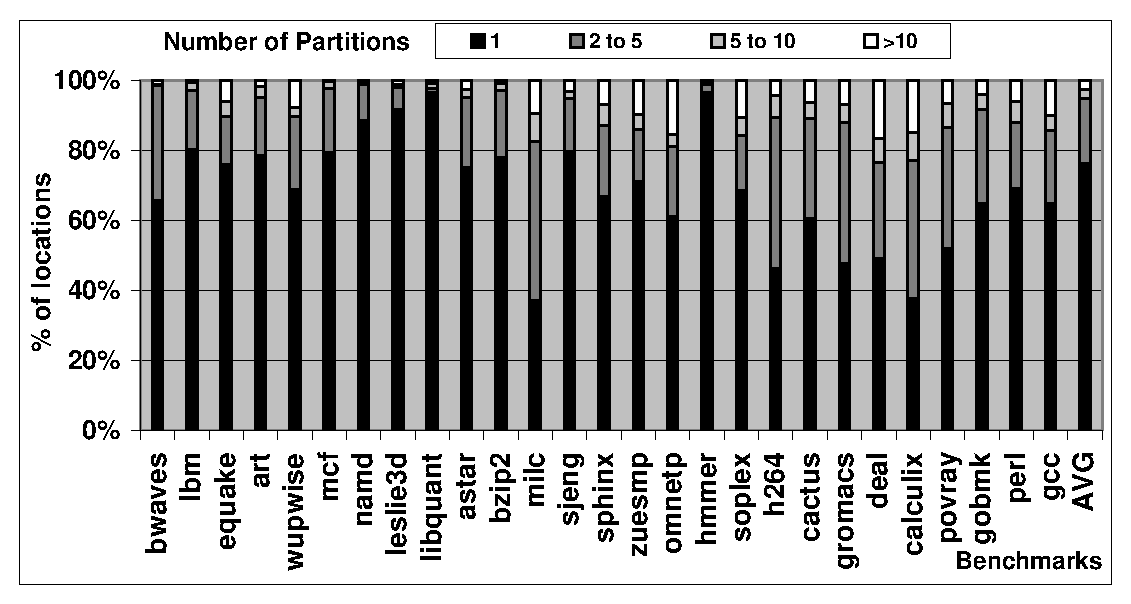
\includegraphics[width=\linewidth]{figures/EPS/partition-visualization.eps}
\caption{\textit{Partition algorithm visualization}}
\label{fig:PartResult}
}
\end{minipage}
\hfill
\begin{minipage}{.29\linewidth}
\centering
{
\begin{tiny}
\begin{tabular}{|c|c|c|c|} %|r|r|r|}
%xxxxx\=xxxxxxxxxxxxx\=xxxxxx\=xxxxxxxxxxx\=xxxxxx\=  \kill\\
\hline
\textbf{Program}&{\textbf{Version}}&{\textbf{Physical stack}}&{\textbf{Run Time}}\\
{}&{}&{}&{\textbf{Checks}}\\ \hline
gcc&gcc-O0,VS-O0&117&0\\\hline
gcc&gcc-O3, VS-Ox&117&10\\	\hline
tonto&gcc-O0, gccO3&20&0\\	\hline
\end{tabular}
\caption {{\textit{Programs demonstrating corner cases of our analysis }}}
\label{fig:resultsCornerCases}
\end{tiny}
%\vspace{-4ex}
}
\end{minipage}
}
\vspace{-3ex}
\end{figure*}
\begin{figure*}[t]
{
%\vspace{-1.2in}
\begin{scriptsize}
%\centering
\begin{minipage}{.35\linewidth}
\centering
{
\includegraphics[width=\linewidth]{figures/EPS/unoptperf.eps}
\begin{scriptsize}
\caption{{ {\textit{Normalized runtime of rewritten binary as compared to unoptimized gcc input binary (=1.0)}}}}
\label{fig:unoptimized}
\end{scriptsize}
}
\end{minipage}
\hfill
\begin{minipage}{.35\linewidth}
\centering
{
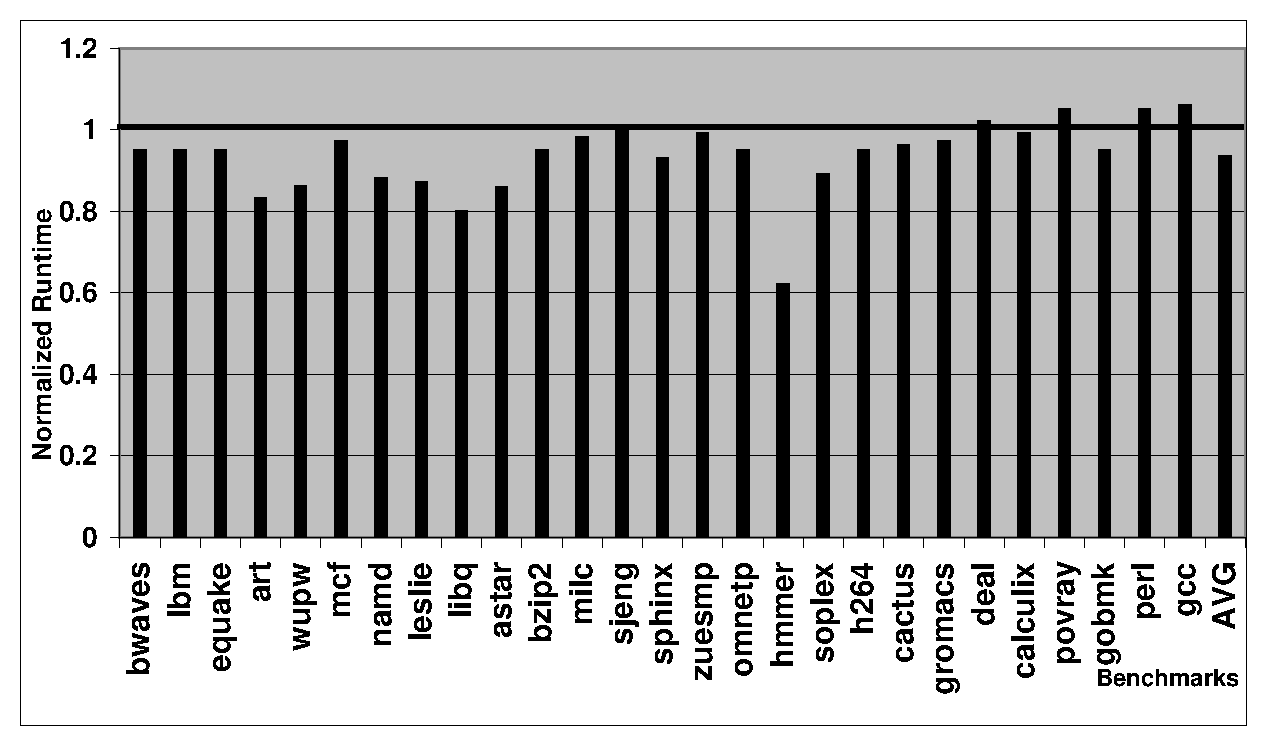
\includegraphics[width=\linewidth]{figures/EPS/optperf.eps}
\begin{scriptsize}
\caption{{{\textit{Normalized runtime of rewritten binary as compared to optimized gcc input binary (=1.0)}}}}
\label{fig:optimized}
\end{scriptsize}
}
\end{minipage} 
\hfill
\begin{minipage}{.28\linewidth}
\centering
{
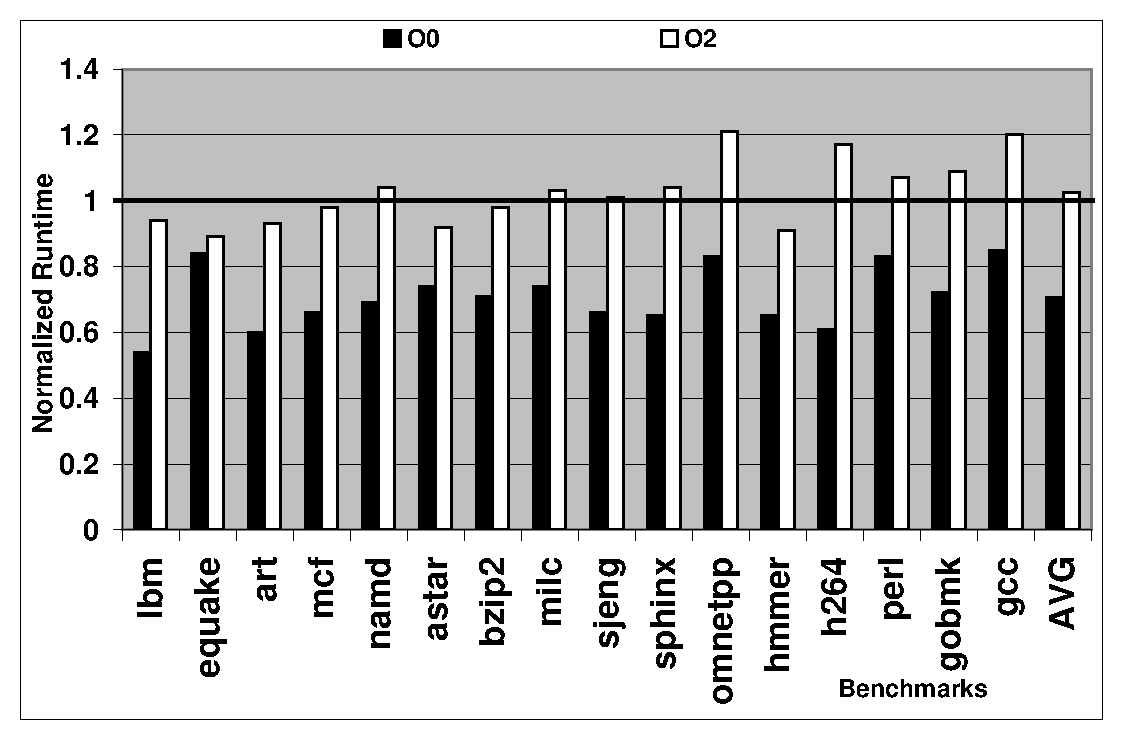
\includegraphics[width=\linewidth]{figures/EPS/pe-binaries.eps}
\begin{scriptsize}
\caption{{{\textit{Normalized runtime of rewritten binary as compared to its corresponding input version (=1.0) compiled by visual studio}}}}
\label{fig:visual-studio}
\end{scriptsize}
}
\end{minipage} 
\end{scriptsize}
}
\vspace{-3ex}
\end{figure*}



Fig~\ref{fig:OrigSymPromResult} relates the above promoted symbolic references to the original source-level artifacts. We enumerated the symbolic references in the input program using debug information (employed only for counting the references) and compared how many of these symbolic references are restored in the IR and the source code. It shows that our techniques are able to restore 66\% of the original symbolic references.

Fig~\ref{fig:PartResult} presents an insightful result regarding our partition algorithm (Alg~\ref{fig:algpartition}). On average, around 76\% of the memory locations have one partition, 18\% have two to five, and 6\% have five or more partitions. This is not unexpected since large procedures are relatively rare.

%the functioning of 
%
\begin{figure}[t]
{
%\vspace{-1in}
\centering
{
\begin{scriptsize}
\begin{tabular}{|c|c|c|c|} %|r|r|r|}
%xxxxx\=xxxxxxxxxxxxx\=xxxxxx\=xxxxxxxxxxx\=xxxxxx\=  \kill\\
\hline
\textbf{Program}&{\textbf{Version}}&{\textbf{Physical stack}}&{\textbf{Run Time Check}}\\ \hline
gcc&gcc-O0,VS-O0&117&0\\\hline
gcc&gcc-O3, VS-Ox&117&10\\	\hline
tonto&gcc-O0, gccO3&20&0\\	\hline
\end{tabular}
\caption {\scriptsize{\textit{Programs demonstrating corner cases of our analysis }}}
\label{fig:resultsCornerCases}
\end{scriptsize}
\vspace{-4ex}
}
}
\end{figure}

Fig~\ref{fig:resultsCornerCases} lists the programs which hit corner cases during the deconstruction of physical stack. The analysis of the original source code revealed that a physical stack frame was required for procedures that call \emph{alloca()}. Runtime checks are inserted in some procedures which accept a variable number of arguments using the \emph{va-arg} mechanism. Most of the procedures using \emph{va-arg} do not require runtime checks. This result establishes our earlier hypothesis that scenarios requiring run-time checks are extremely rare and consequently, have negligible overhead. Nonetheless, not handling these scenarios prohibits obtaining a functional IR and hence, are imperative for any translation system.

%\vspace{-3ex}
\subsection{Un-optimized input binaries}
Fig~\ref{fig:unoptimized} shows the normalized run-time of each rewritten binary compared to an input binary produced using gcc with no optimization (-O0 flag). Fig~\ref{fig:visual-studio} shows the corresponding run-time for binaries produced using Visual Studio compiler with no optimization (-O0 flag). We obtain an average improvement of 40\% in execution time for binaries produced by gcc and 30\% for binaries produced by Visual Studio, with an improvement of over 65\% in some cases (\emph{bwaves}). In fact, our tool brings down the normalized runtime of unoptimized input binaries from 2.2 to close to the runtime (1.25) of gcc-optimized binaries. (Graph not shown due to lack of space)
%his result shows that our rewriter is very useful for binaries that are not highly optimized.
%, such as legacy binaries(Graph not shown due to lack of space) %Fig~\ref{fig:unopt-cmp} compares the run-time of un-optimized input binary and the corresponding rewritten binary with an optimized binary produced directly by gcc. or binaries from compilers that are inferior compared to the today's best available compilers. 
%
%\footnote{We started experimenting with visual-studio binaries only recently and have presented the results for all the binaries which have been rewritten correctly. The runtime results are presented for visual studio binaries to demonstrate that our schemes are not compiler-dependent. Detailed experimental results are presented for gcc-produced binaries} 
%In most cases, after rewriting we raised the performance close to that of an optimized binary produced directly by gcc, showing the effectiveness of our approach.
%\input{figures/unoptperf}


\begin{figure*}[t]
{
%\centering
\vspace{-0.33in}
{
%\begin{minipage}[t]{.31\linewidth}
%\centering
%{
%\includegraphics[width= 2.3 in]{figures/EPS/unopt-optcomp.eps}
%\caption{{\textit{Normalized runtime of unoptimized input binary and its rewritten version as compared to optimized input binary(=1.0)}}}
%\label{fig:unopt-cmp}
%}
%\end{minipage}
%\hfill
\begin{minipage}{.35\linewidth}
\centering
{
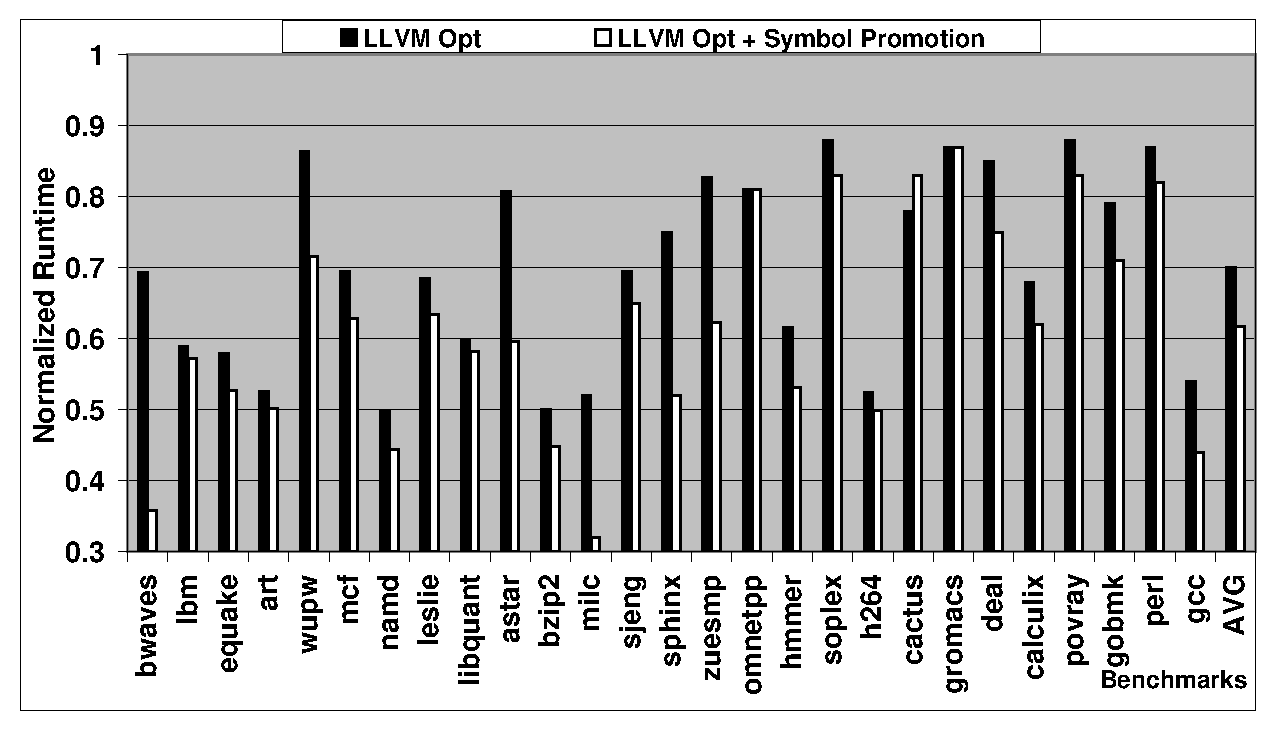
\includegraphics[width=\linewidth]{figures/EPS/impactunopt.eps}
\caption{{\textit{Impact of symbol promotion on runtime of rewritten binary v/s unoptimized input binary (=1.0) }}}
\label{fig:unopt-symprom}
}
\end{minipage}
\hfill 
\begin{minipage}{.35\linewidth}
\centering
{
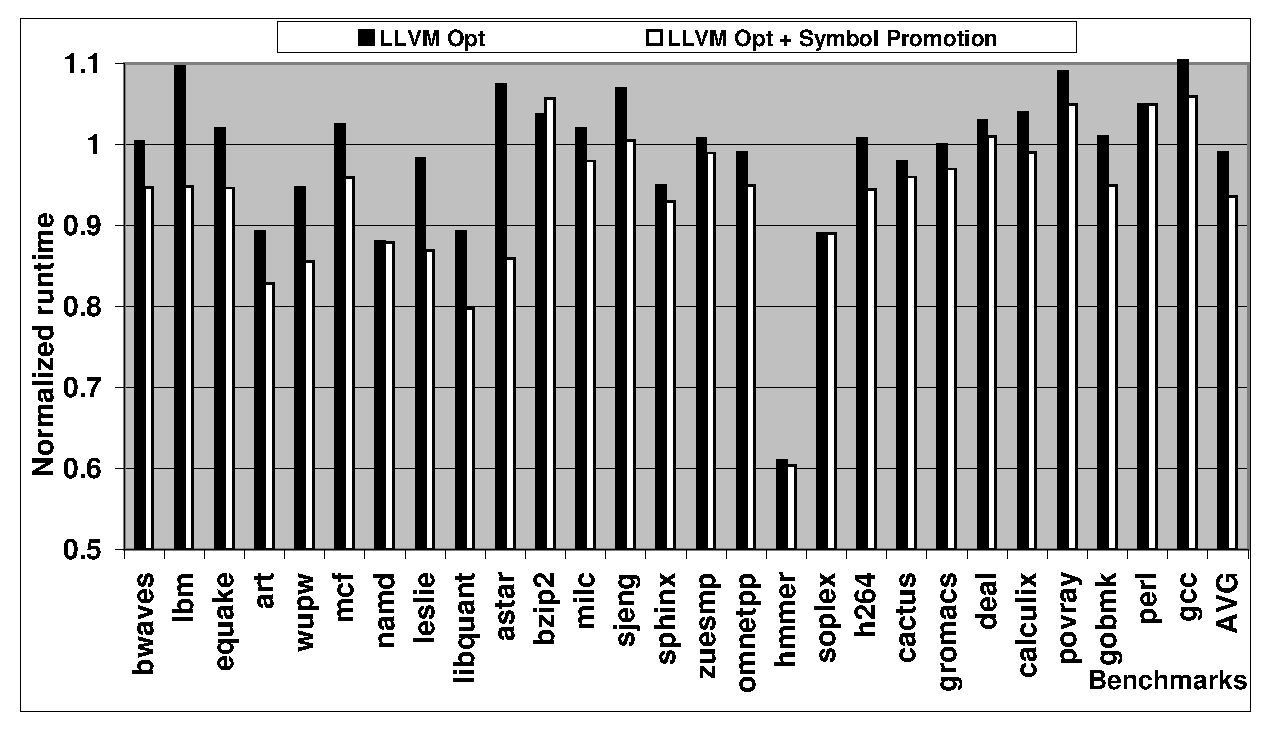
\includegraphics[width=\linewidth]{figures/EPS/impactopt.eps}
\caption{{\textit{Impact of symbol promotion on runtime of rewritten binary v/s optimized input binary (=1.0)}}}
\label{fig:opt-symprom}
}
\end{minipage}
\begin{minipage}{.29\linewidth}
\centering
{
\includegraphics[width=\linewidth]{figures/EPS/klee-coverage.eps}
\caption{{\textit{Normalized code coverage in coreutils binaries as compared to source }}}
\label{fig:KleeCovRes}
}
\end{minipage}
}
\vspace{-4ex}
}
\end{figure*}


\begin{figure*}[t]
{
%\vspace{-0.2in}

%\centering
{
%\begin{minipage}[t]{.31\linewidth}
%\centering
%{
%\includegraphics[width=2.1in]{figures/EPS/klee-coverage.eps}
%\caption{\scriptsize{\textit{Normalized code coverage in coreutils binaries as compared to source }}}
%\label{fig:KleeCovRes}
%}
%\end{minipage}

\begin{minipage}{.24\linewidth}
%\centering
{
\begin{scriptsize}
\begin{tabular}{|l|l|} %|r|r|r|}
%xxxxx\=xxxxxxxxxxxxx\=xxxxxx\=xxxxxxxxxxx\=xxxxxx\=  \kill\\
\hline
{mkdir -Z a b}&{mkdir -Z @@ -}\\ 
{mkfifo -Z a b}&{mkfifo -Z @@ -}\\ 
{mknod -Z a b p}&{mkdir -Z @@ - p@}\\ 
{seq -f \%0 1}&{seq -f \%1 1}\\ 
{paste -d\textbackslash \textbackslash   }&{paste -d\textbackslash \textbackslash   }\\ 
{\hspace{1ex}abcdefghijklmn}&{\hspace{1ex}@@@@@@@@ }\\ 
{}&{\hspace{1ex}@@@@@@ }\\  \hline
\end{tabular}
\caption {{\textit{Testcases for crashes (a)Source code~\cite{Cadar-KLEE} (b) Binaries }}}
\label{fig:result-symExec-testCases}
\end{scriptsize}%\vspace{-4ex}
}
\end{minipage}
%\begin{minipage}{.24\linewidth}
%\centering
%{
%\includegraphics[width=\linewidth]{figures/EPS/resultssymExecution-testCase.eps}
%\caption{{\textit{Test cases for crashes (a) Source code (b) Binaries}}}
%\label{fig:result-symExec-testCases}
%}
%\end{minipage}
\hfill
\hspace{1ex}
\begin{minipage}{.21\linewidth}
\centering
{
\begin{scriptsize}
\begin{tabular}{|l|l|l|} %|r|r|r|}
%xxxxx\=xxxxxxxxxxxxx\=xxxxxx\=xxxxxxxxxxx\=xxxxxx\=  \kill\\
\hline
{Binary}&{No}&{With}\\ 
{}&{Promotion}&{Promotion}\\ \hline
htget&980&4671\\ \hline
cut&1301&5103\\ \hline
split&1623&4104\\ \hline
\end{tabular}
\caption {{\textit{Improvement in constraints processing with symbol promotion }}}
\label{fig:results-symExecSymMem}
\end{scriptsize}%\vspace{-4ex}
}
\end{minipage}
\hfill
\hspace{1ex}
\begin{minipage}{.24\linewidth}
\centering
{
\includegraphics[width=\linewidth]{figures/EPS/parallel-runtime.eps}
\caption{{\textit{Automatic parallelization}}}
\label{fig:parallel-runtime}
}
\end{minipage} 
\hfill
%\hspace{-2ex}
\begin{minipage}{.24\linewidth}
\centering
{
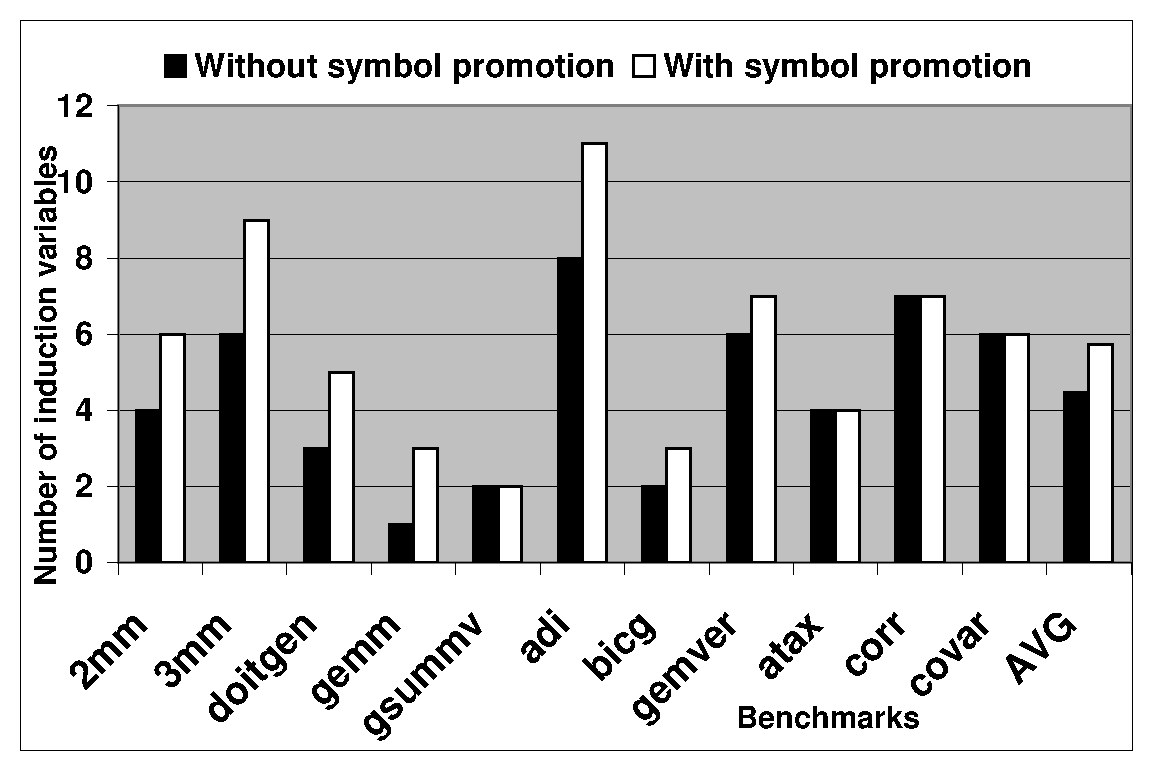
\includegraphics[width=\linewidth]{figures/EPS/induction-var.eps}
\caption{{\textit{Number of induction variables recognized}}}
\label{fig:parallel-indvar}
}
\end{minipage}
}
\vspace{-3ex}
}
\end{figure*}


\subsection{Optimized input binaries}
Fig~\ref{fig:optimized} shows the normalized execution time of each rewritten binary compared to an input binary produced using gcc with the highest-available level of optimization (-O3 flag). In this case, we obtain an average improvement of 6.5\% in execution time. It is interesting that we were able to obtain this improvement over already optimized binaries without any custom optimization of our own. One of our rewritten binaries (hmmer) had a 38\% speedup vs the input binary. Although GCC -O3 is known to produce good code, it missed the creation of few predicated instructions whereas LLVM did this optimization, explaining the speedup. Fig~\ref{fig:visual-studio} shows the corresponding run-time for binaries produced using Visual Studio compiler with full optimization flag (-O2). As evident, our framework was able to retain the performance of these binaries, with a small overhead of 2.7\% on average. 
%It exemplifies the underlying advantage of our binary rewriter - that it cumulates optimizations across two compilers -- rewritten binaries have an optimization if it is either present in the compiler that produced the input binary, or in the rewriter. This is why, for example, one of our rewritten binaries (hmmer) had a 38\% speedup vs the input binary. Although GCC -O3 is known to produce good code, it missed the creation of few predicated instructions whereas LLVM did this optimization, explaining the speedup. 
%In our case, if either GCC or LLVM had an optimization, the output binary should have it. , with one benchmark actually showing up a speedup of 38\% (hmmer)

%\input{figures/impact-symbol}
%\vspace{-2ex}
\subsection{Impact of symbol promotion}
Next, we substantiate the impact of symbol promotion on the run-time of rewritten binaries. Fig~\ref{fig:unopt-symprom} and Fig~\ref{fig:opt-symprom} show the normalized improvement in execution time obtained by applying only LLVM optimizations and by applying our symbol promotion techniques. It shows that symbol promotion is responsible for improving the average performance of rewritten binary from 30\% to 40\% in the case of unoptimized binaries (produced by gcc) and from 1\% to 6.5\% in the case of optimized binaries (produced by gcc). Since our cost metric is based on static profiling, we observed a small slowdown with symbol promotion in \emph{bzip2 O3}. 
%one of our benchmark 
%We reckon that symbol promotion accelerates the binaries in two ways: first, it serves as an implicit load-store forwarding optimization and secondly, it improves the efficiency of other optimizations. This result captures the combined effect of symbol promotion.

It is important to note that these results only measure the impact of symbol promotion. The impact of our method to convert physical frames to abstract frames is not measured above. However, we can infer that number since without obtaining abstract frames, none of the existing LLVM passes would run at all, leading to zero run-time improvement.	

%Fig~\ref{fig:static-impact} helps in quantifying the impact of symbol promotion on efficiency of individual compiler analysis. We chose three compiler analysis - copy propagation, constant propagation and dead-code elimination and collected their static performance statistics with and without the presence of symbols for three of our benchmarks. Fig~\ref{fig:static-impact} shows the normalized improvement in the number of static instances of each of these optimizations when using symbol promotion. Symbol promotion allows the compiler's copy propagation pass to implicitly implement store-load forwarding, explaining a large increase in copy propagation statistics. The effectiveness of other optimizations also improves considerably with the presence of symbols in the IR. 
 %hence the data for copy propagation has been scaled down by 10 to fit in the graph.

%Symbol promotion helps us in improving the quality of IR in general and makes it more suitable for analysis purposes. We analyze this subjective improvement by showing its impact on the C code obtained by compiler backend for ease of understanding. Fig~\ref{} shows an original C code and C code obtained from the binary with and without symbol promotion. As evident from this figure, the C code obtained after doing symbol promotion is more closer to the original source code. Having such detailed representation in C code would improve the existing analysis frameworks for binaries with no source code e.g. legacy binaries.

\subsection{Symbolic Execution}

%%\begin{figure}[t]
%\vspace{-0.5in}
%\centering
%\psfig{figure=figures/plots/runtimeFinal.eps,width=5.5in} }
%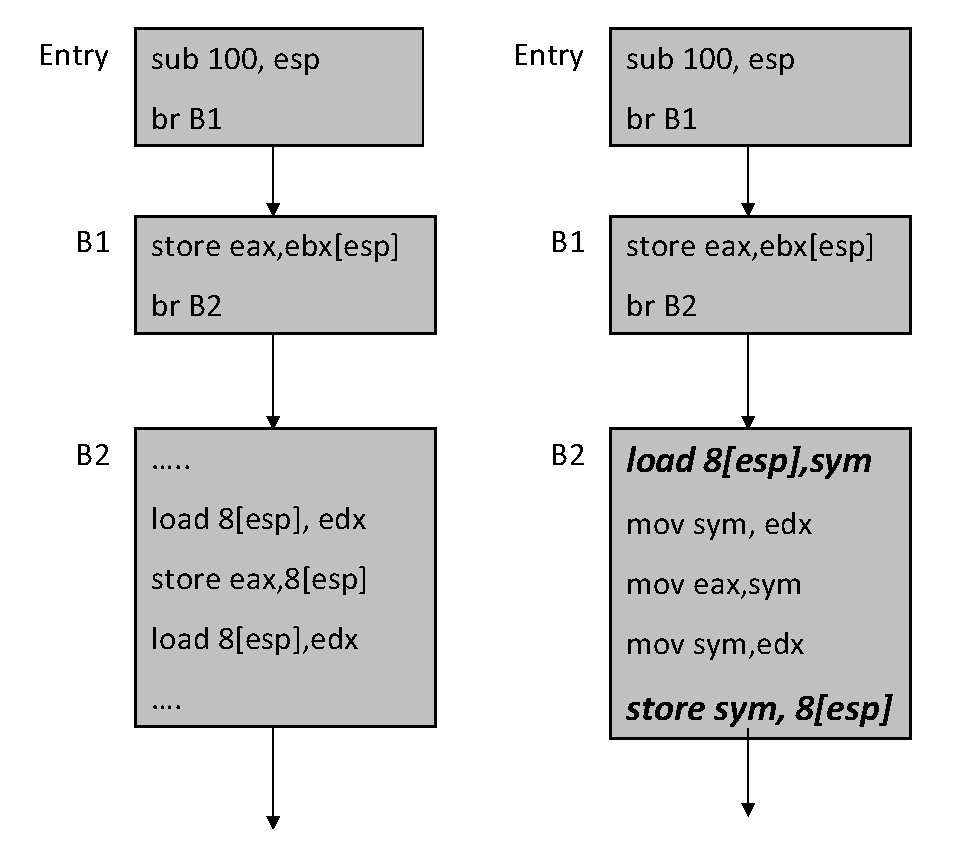
\includegraphics [width=0.5\linewidth] {figures/EPS/cfgex.eps} 
%\tiny{
%\caption { \textit{Stack layout in a binary}}
%}
%\label{fig:stack-layout}
%\end{figure}

\begin{figure}[b]
{
\vspace{-2ex}
\centering
\includegraphics[width=0.6\linewidth]{figures/EPS/klee-coverage.eps}
\caption{\textit{Normalized code coverage in coreutils binaries as compared to source }}
\label{fig:KleeCovRes}
}
%\hfill
\vspace{-5ex}
\end{figure}




%\begin{figure}[t]
%{
%\centering
%\begin{minipage}{.6\linewidth}
%{
%\centering
%\includegraphics[width=0.5\linewidth]{figures/EPS/pathcfg.eps}
%\caption{\textit{Path dependent promotion. Second operand in the instruction is the destination of the instruction. }}
%\label{fig:PromExample}
%}
%\vspace{-0.1in}
%\end{minipage}
%%\hfill
%\begin{minipage}{0.3\linewidth}
%{
%\centering
%\includegraphics[width=0.3\linewidth]{figures/EPS/partitioncfg.eps} 
%\caption{\textit{Motivation for partition}}
%\label{fig:PartExample}
%}
%\vspace{-0.1in}
%\end{minipage}
%}
%\vspace{-0.2in}
%\end{figure}

%Code coverage
KLEE is efficiently designed to obtain a high code coverage on source programs. We run KLEE in our framework on a set of 50 coreutils binaries and compare the resulting code coverage with that achieved by KLEE on the corresponding source code in Fig~\ref{fig:KleeCovRes}. Our framework achieves a code coverage of 73\% on average compared to 76\% obtained by KLEE on source programs. 
%This experiment demonstrates that symbolic execution using KLEE on the IR produced by our framework achieves almost similar coverage as it achieves on source code.

%\begin{figure}[t]
{
%\vspace{-1in}
\centering
\includegraphics[width=0.5\linewidth]{figures/EPS/resultssymExecution-testCase.eps}
\vspace{-3ex}
\caption{\textit{KLEE generated test cases for crashes in coreutils (a) Source code (as reported by KLEE paper) (b) Binaries (Generted in our framework)}}
\label{fig:result-symExec-testCases}
}
\vspace{-4ex}
\end{figure}

%bug detection
KLEE has been shown to detect various bugs in a particular version of coreutils (6.10). Fig~\ref{fig:result-symExec-testCases} lists the test cases generated through our framework and those reported in the original KLEE paper\footnote{The original KLEE paper shows 10 bugs in coreutils but latest version of KLEE only detects five of these bugs}. Note that the original KLEE paper detected these bugs from source code, but our framework detected the same bugs from binaries. Both these results demonstrate the unique ability of our framework to efficiently employ source level research directly for executables. 
%This shows that our framework is able to reliably detect the bugs which are detected by directly applying symbolic execution of source code., and generate corresponding test cases for each detected bug,

%\begin{figure}[t]
{
\begin{minipage}[t]{.4\linewidth}
\centering
{
\begin{scriptsize}
\begin{tabular}{|c|c|c|} %|r|r|r|}
%xxxxx\=xxxxxxxxxxxxx\=xxxxxx\=xxxxxxxxxxx\=xxxxxx\=  \kill\\
\hline
{Binary}&{No}&{With}\\ 
{}&{Promotion}&{Promotion}\\ \hline
htget&980&4671\\ \hline
cut&1301&5103\\ \hline
split&1623&4104\\ \hline
\end{tabular}
\caption {\scriptsize{\textit{Improvement in constraints processing with symbol promotion }}}
\label{fig:results-symExecSymMem}
\end{scriptsize}%\vspace{-4ex}
}
\end{minipage}
\hfill
\begin{minipage}[t]{.5\linewidth}
\centering
{
\includegraphics[width=\linewidth]{figures/EPS/resultssymExecution-testCase.eps}
\caption{\scriptsize{\textit{Test cases for crashes in coreutils (a) Source code (KLEE paper) (b) Binaries (Our framework)}}}
\label{fig:result-symExec-testCases}
}
\end{minipage}
}
\vspace{-4ex}
\end{figure}

%symbolic memory
Recall from Sec~\ref{sec:symExec}, symbol promotion enables our framework to efficiently reason about symbolic memory accesses. We run symbolic execution on IR produced from binaries for 30 minutes and compare the result in two scenarios: with and without symbol promotion. Fig~\ref{fig:results-symExecSymMem} shows that the presence of symbol promotion greatly improves the number of constraints processed by the solver, resulting in a much higher code coverage in the same amount of time. Program \emph{htget} has been shown to have a bug~\cite{Brumley-Mayhem} and we were able to detect that bug within 5 minutes in the presence of symbols as opposed to 25 minutes without symbol promotion.
%\footnote{KLEE simulates symbolic memory for only concrete-size memory objects, hence, variable-sized memory allocations in the above programs had to be replaced by fixed size allocations.}
%bug fix

Further, the presence of a rewriting path in our framework enables us to remedy the above detected bugs in binaries. We analyzed the dump for one of the coreutil binary (\emph{mkdir}), fixed the corresponding behavior in IR and obtained a rewritten bug-free binary.
%    us application synergizing the symbolic execution and rewriting path of our framework. As evident from Fig~\ref{fig:result-symExec-testCases}, KLEE detects a bug in mkdir coreutil binary. Analysis of the dump revealed that the error arises when an invalid global location is passed to a print function. We were able to fix this behaviour in IR and obtained a rewritten binary which didn't display this bug.

%Next, we demonstrate an interesting application synergizing the symbolic execution and rewriting path of our framework. As evident from Fig~\ref{fig:result-symExec-testCases}, KLEE detects a bug in mkdir coreutil binary. Analysis of the dump revealed that the error arises when an invalid global location is passed to a print function. We were able to fix this behaviour in IR and obtained a rewritten binary which didn't display this bug.

%Fig~\ref{} shows the corresponding dump in case of mkdir coreutil. 
%The original KLEE framework dumps the location of each detected bug in the input source code. Since a standalone binary does not contain debug information, we modified KLEE to dump the corresponding buggy location in LLVM IR. In fact, the original error as reported by KLEE in mkdir is related to \emph{optarg} being passed as emph{NULL}.

\subsection{Automatic Parallelization}
Kotha et al~\cite{micro-aparna10} presented a method for automatic parallelization for binaries. Here, we substantiate the impact of symbol promotion on their methods for a subset of \emph{PolyBench} and \emph{Stream} suite. Fig~\ref{fig:parallel-runtime} shows that symbol promotion increases the speedup by 2.25x for 4 threads.
%of 11 benchmarks

The underlying reason for the speedup is that symbol promotion enables discovery of more induction variables. Many induction variables for outer loops are often present on the stack instead of registers. Consequently, such induction variables are not detected by compiler methods, resulting in parallelization of inner loops, which have high synchronization overhead. As shown in Fig~\ref{fig:parallel-indvar}, symbol promotion enables the discovery of more induction variables, enabling the parallelization of more beneficial outer loops.

%We further investigate why symbol promotion helped automatic parallelization significantly. In order to parallelize loops using an affine automatic parallelizer, it is essential to recognize induction variables. We observe that for x86 binaries, many induction variables, for affine loops of nesting depth greater than two, are often present on the stack instead of registers;  the compiler's induction variable recognizer based on symbols fails to recognize them. This results in parallelization of only inner loops even though outer-loop parallelization is legal. Parallelizing inner loops involves a significant synchronization overhead resulting in a lower speedup. On the other hand, symbol promotion promotes the stack allocated-induction variables corresponding to outer loops also to symbols; consequently, these induction variables get recognized and it allows the parallelizer to do parallelization on more beneficial outer loops. Fig~\ref{fig:parallel-indvar} shows the number of outer loops for which induction variables are recognized with and without symbol promotion.
%Further, for affine loops of nesting depth greater than two, induction variables of outer loops are generally placed on the stack. 

%hence we parallelize inner loops when symbol promotion is not performed even though outer-loop parallelization is legal
%In affine loops of nesting depth greater than two, induction variables of outer loops are generally placed on the stack since there are no free registers for them. To parallelize these loops using the most basic affine automatic parallelizer on binaries, it is essential to recognize these locations on stack and promote them to variables, which will enable the compiler's induction variable recognizer to recognize them as induction variables. We observe that for x86 binaries compiled using gcc -O3 many induction variables are often present on the stack and hence we parallelize inner loops when symbol promotion is not performed even though outer-loop parallelization is legal. Parallelizing inner loops implies that there is a significant overhead due to synchronization and hence the speedup is lower than the case when symbol promotion is performed. A detailed statistics of number of outer loops for which induction variables recognized with and without symbol promotion is presented in figure~\ref{fig:parallel-indvar}. 

%We conclude by associating the advantages of a compiler IR based rewriter listed in ~\ref{sec:intro} with our results. Automatic parallelization and security enforcements depict that compiler IR allows any complex code transformation in a rewriter as well as ability to reuse compiler research methods. Further, the application of existing LLVM compiler analysis depict the reuse of compiler passes. The improvement in induction variable recognition and alias analysis show that the compiler analysis perform better with presence of symbols. Also, the better quality of C code show that presence of symbols make IR more favorable to analysis. In future work, we would 
\section{Related Work}\label{sec:relwork}

The traditional method of compiler loop optimizations including loop peeling, loop reversal, and loop interchange has been applied to code generation for distributed memory multiprocessors \cite{callahan1988compiling, ramanujam1991compile}. These techniques are useful for discovering parallelism, improving the granularity of parallelism, and improving cache performance. However, Chapel is an explicitly parallel language, and the degree of parallelism is already defined by the programmer. Furthermore, these methods require footprint calculations which are modeled by matrices and need to be intersected with the data distribution in order to provide code generation for message passing machines. Our method does not require any footprint calculations, thereby simplifying code generation. 

The polyhedral method is another branch of compiler optimization that seeks to speed up parallel programs on distributed memory architectures \cite{chavarria2005effective, germain1995automatic, Gupta91automaticdata, gupta1996compiling, iancu2008performance, wei1998compiling}. In this method, boundaries are traced for each array use and these are intersected with the program's data distribution. A detailed mathematical framework to express parallelism and find sequences of transformations can occur in one step using this method. However, the method at its core does not compute information for message passing code generation. 

Similar work to take advantage of communication aggregation on distributed arrays has already been done in Chapel. In \cite{sanz2012global}, aggregation was applied to improve the communication performance of whole array assignments for Chapel's Block and Cyclic distributions. Our work goes beyond array assignments and is applicable to affine array accesses within parallel loops for Chapel's Cyclic and Block Cyclic distributions. One of the contribution's of \cite{sanz2012global} included two new bulk communication primitives for Chapel developers, \texttt{chpl\_comm\_gets} and \texttt{chpl\_comm\_puts}. They both rely on the GASNet networking layer, a portion of the Chapel runtime.  Modulo unrolling takes advantage of these new communication primitives to perform bulk remote data transfer between locales.

Extensive work has been done with the UPC compiler (another PGAS language) by \cite{chen2005communication} to improve on communication performance. This method targets fine-grained communication and uses techniques such as redundancy elimination, split-phase communication, and communication coalescing to reduce overall communication. However, there is no locality analysis that statically determines whether an array access is shared or remote. Our method, modulo unrolling, can determine which accesses are local purely on the affine array access and data distribution. 

\begin{comment}
\cite{callahan1988compiling}
\cite{chamberlain1998zpl}
\cite{chamberlain1997factor}
\cite{chavarria2005effective}
\cite{davidson1995improving}
\cite{Dion96compilingaffine}
\cite{germain1995automatic}
\cite{Gupta91automaticdata}
\cite{gupta1996compiling}
\cite{huang1994speculative}
\cite{iancu2008performance}
\cite{li1991data}
\cite{pouchet2011loop}
\cite{ramanujam1991compile}
\cite{shih2000efficient}
\cite{trifunovic2010graphite}
\cite{wei1998compiling}
\cite{chamberlain2011user}
\cite{bonachea2007proposal}
\cite{sanz2012global}
\end{comment}

%\begin{singlespace}
%\begin{scriptsize}

{
%\def\bibfont{\footnotesize}
%\bibliographystyle{ieee}
\begin{singlespace}
%\begin{scriptsize}
%\begin{footnotesize}
\vspace{-3ex}
\bibliography{bibliography}
\vspace{-2ex}
\bibliographystyle{abbrv}
%\bibliography{matt}
%\end{scriptsize}
\end{singlespace}
}

%\setlength{\bibspacing}{\baselineskip}
%\bibliography{angelos,references,local,extra,nghi,kiran,matt,mincy,kiran2,RewriterSurveyReferences,karan,selfmod}
%\bibliographystyle{plain}
%\end{scriptsize}
%\end{singlespace}
%\newpage
%\pagestyle{empty}
%\input{facilities}

%\newpage
%\pagestyle{empty}
%\input{mentoring}

\end{document}
